\documentclass[a4paper,11pt]{article}
\addtolength{\textwidth}{1.5in}
\addtolength{\hoffset}{-0.75in}
\usepackage{subfigure}
%\addtolength{\textheight}{0.5in}
%\addtolength{\voffset}{-0.25in}
\usepackage{rotating}
\usepackage{comment}
\usepackage{english}
\usepackage[T1]{fontenc}
\usepackage[latin1]{inputenc}
\usepackage{hyperref}
\usepackage{amsmath}
\usepackage{graphicx}
\usepackage{fancyhdr}
\usepackage{graphicx}
\usepackage{minipage}
\usepackage{listings}
\lstset{language=Matlab}
\pagestyle{fancy}
\lhead{}
\chead{}
\rhead{}
\lfoot{}
\cfoot{}
\rfoot{\thepage}
\title{\textbf{\huge{Artificial neural networks - Lab 2}}}
%\author{Magnus Raunio, 900531-5131}
\selectlanguage{english}

\begin{document}

\maketitle

\section{Theory}

\begin{itemize}

\item \textit{What is the lower bound for the number of training examples, N?} \\
N needs to be atleast n + 1 since otherwise we can solve the equation exactly.

\item \textit{What happens with the error if N = n? Why?} \\
In theory we will get a zero error since we can solve the equation exactly and it's no longer overdetermined.

\item \textit{Under what conditions, if any, does (4) have a solution in this case?}  \\
The equation has a solution for N <= n since we have more/equal weights than approximation values and we can tune the weights to solve the equation.

\item \textit{During training we use an error measure dened over the training exam ples. Is it good to use this measure when evaluating the performance of the network? Explain!} \\
It's good to see if the network is working, but to measure the performance of the network we should use a valdiation set which we approximate and measure the error for. Since the network is trained on the training data and it's minimizing the error for the training data it will get a good result for the trainig data but it does not neccesarily reflect the perforamce it will have on different data. If we train to much we may overfitt the network for the training data.
\end{itemize}
\section{Least square}
\begin{itemize}

\item \textit{How many units did you require to get down to a maximum (absolute) residual value of 0.1, 0.01 and 0.001?} \\
7,25,56

\begin{figure}[h!]
\subfigure[Run to get error below 0.1]{
    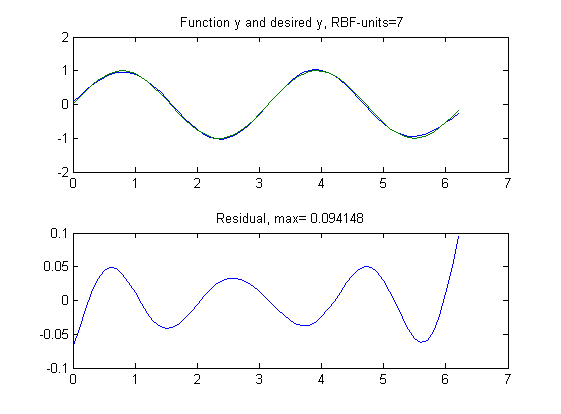
\includegraphics[width=0.5\linewidth]{lab2/sin2x_under1.png}
    \label{fig1:sub1}
}
\subfigure[Run to get error below 0.01]{
    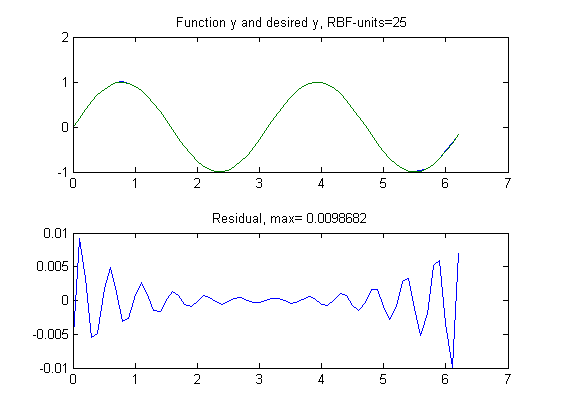
\includegraphics[width=0.5\linewidth]{lab2/sin2x_under01.png}
    \label{fig1:sub2}
}
\subfigure[Run to get error below 0.001]{
    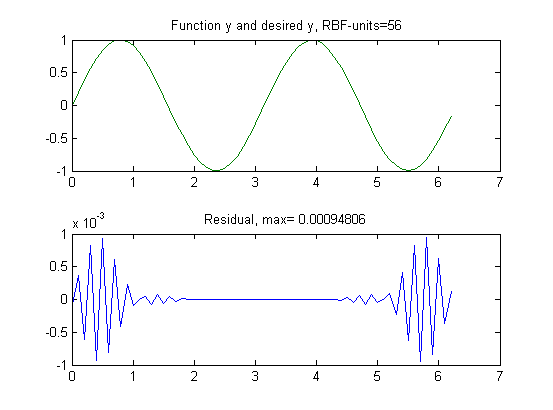
\includegraphics[width=0.5\linewidth]{lab2/sin2x_under001.png}
    \label{fig1:sub4}
}
\label{fig1}
\caption{}
\end{figure}

\item \textit{Give a good reason for the big difference in residual between 5 and 6 units for sin(2x).}  \\
We need one node to represent each peak and valley aswell as two extra nodes to represent the end and start points to be able to approximate the function exactly. If we look at the weight matrix for the 6 units RBF network we also see that the weights have switched signs for the next weights to reflect the fact that we have a function which is periodic.

\begin{figure}[h!]
\subfigure[Run with 5 hidden units]{
    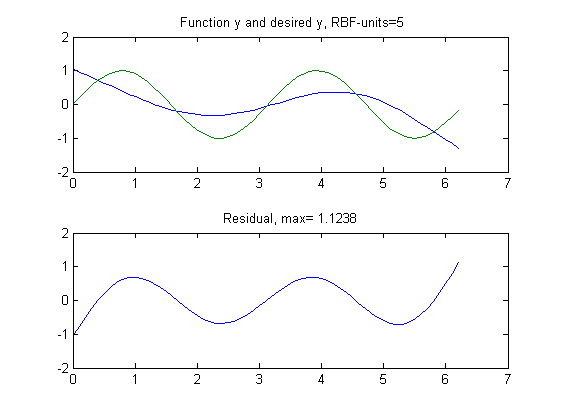
\includegraphics[width=0.5\linewidth]{lab2/sin2x_5units.png}
    \label{fig2:sub1}
}
\subfigure[Run with 6 hidden units]{
    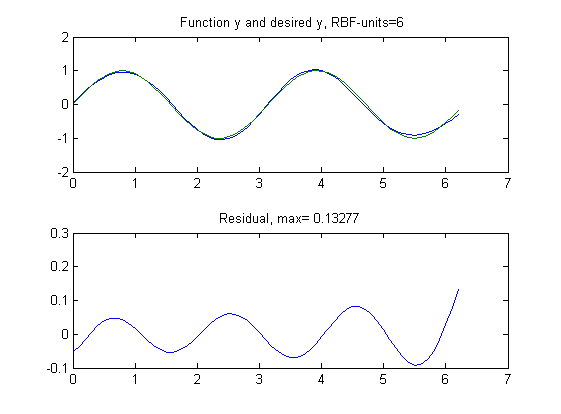
\includegraphics[width=0.5\linewidth]{lab2/sin2x_6units.png}
    \label{fig2:sub2}
}
\subfigure[Transfer functions for the run with 5 units]{
    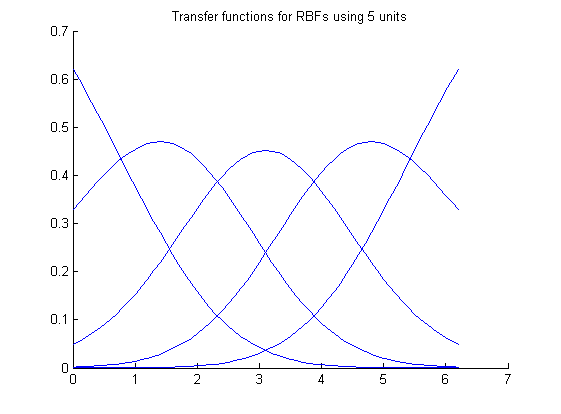
\includegraphics[width=0.5\linewidth]{lab2/sin2x5.png}
    \label{fig2:sub3}
}
\subfigure[Transfer functions for the run with 6 units]{
    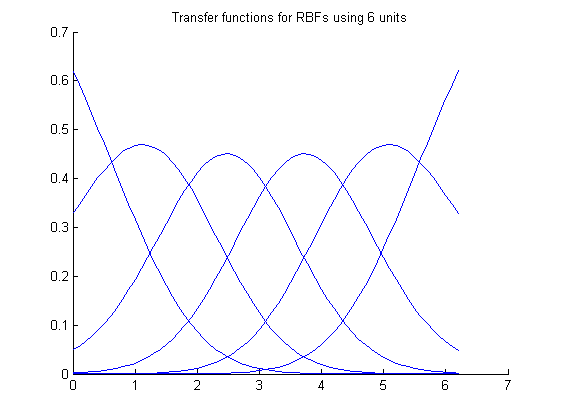
\includegraphics[width=0.5\linewidth]{lab2/sin2x6.png}
    \label{fig2:sub4}
}

\label{fig2}
\caption{}
\end{figure}

\item \textit{How many units did you require, when approximating square(2x),to come down to residual values of 0.1, 0.01 and 0.001?}

We needed 59 or 62 nodes to get under 0.1 and 63 for both 0.01 and 0.001. 63 is the number of datapoitns which we are training on though so ofcourse we get a very small error then since we can match them ''exactly'' when we have as many hidden nodes as datapoints. Apperently the RBF netowkr works better for smooth functions.

\item \textit{Approximating square(2x) is a somewhat special case of function approximation since it is similar to another area of use for artificial neural networks. Which? Hint: ANNs can be used for pattenr completion, noise reduction...}

Based on the hints it's probably signal processing that is the area of use we're looking for. We can see it as if we're approximating a binary signal after all.

\item \textit{Can you, with a suitable action (e.g. transforming network output), easy get down (for training values) to a residual value=0? What action? How many units did you require?}

We can threashold units so that they are either 1 or -1 with the sign function. We require 6 hidden units since that's what is needed to approximate a sin wave of the same periodicity.

\item \textit{Can an RBF network solve the XOR problem? If not, explain why not. If yes, explain how.}

The lab notes seem to say that we can classify non lineraly seperable data with RBF:s, see page 3, top of page right before section 3.2. More specifically we need to get one output for (0,0) and (1,1) and one output for (1,0) and (0,1). If we center two gaussians of the same size on (0,0) and (1,1) we will get two max peaks at (0,0) and (1,1) and since (1,0) and (0,1) are in between them we will get a lower value for those two points. Thus we have mapped (0,0) and (1,1) to one value and (1,0) and (0,1) to another value.
\end{itemize}

\section{Delta rule}
\begin{itemize}

\item \textit{How many units and iterations did you require to come down to a maximum residual value of 0.01 when using the delta rule? What value(s) of eta did you use?}

A combination of 500000 iterations, eta = 0.05 and 50 units got us an error below 0.01. Perhaps try again with higher eta and lower iterations to make it faster.
Seems like this was too much though, but it was hard to get from 0.1 to 0.01

with eta = 1, 35unit and 100,000 iteration we are close to 0.013
I think that our evaluating of the error is wrong, we should not evaluate the error on the edge (close tu 0 and 2 pi)










\item \textit{Now try approximating some function of your own choice. Use least squares or the delta rule as you wish.}

We approximate a lienar function and a sqrt function. In the lienar function we see that the RBF works better for periodic functions since we see ''waves'' around the linear line as if the line was periodic.

\begin{figure}[h!]
\subfigure[Lineaarly approximated function]{
    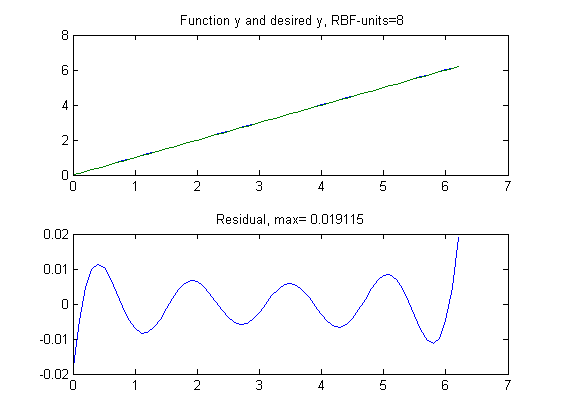
\includegraphics[width=0.5\linewidth]{lab2/linear.png}
    \label{fig3:sub1}
}
\subfigure[$sqrt(x)$ approximated function]{
    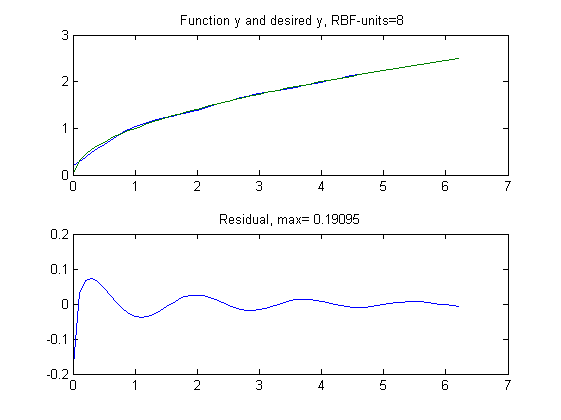
\includegraphics[width=0.5\linewidth]{lab2/sqrt.png}
    \label{fig3:sub2}
}

\label{fig3}
\caption{}
\end{figure}
\end{itemize}

\section{VQ and EM}
\begin{itemize}

\item \textit{What problem could be seen when using the single winner strategy (singlewinner=1)?}

%We don't actually have a a nieghbourhood so we only have self organization and not self organisating maps.
%Either everyone gets some or only one gets some.
We could see that some units never won and were left out and therby became dead nodes which serves no function in the network. This is mostly a problem when a node tries to take many datapoints but they don't really fall within the area of it's transfer function. If you had used the dead nodes you could have captured the other datapoints aswell.

\begin{figure}[h!]
\subfigure[Vector Quantization with a single winner. We have one dead unit.]{
    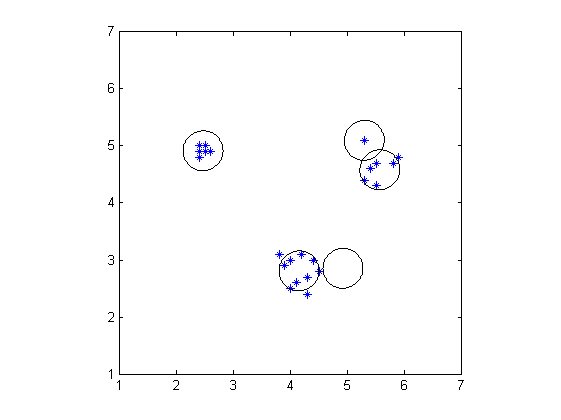
\includegraphics[width=0.5\linewidth]{lab2/vqOk2.png}
    \label{fig4:sub1}
}
\label{fig4}
\caption{}
\end{figure}

\item \textit{What is the advantage of using this strategy?}

The advantage of using a single winner is that you can remove the dead nodes and thereby get a smaller network.

\item \textit{Describe differences between using the single winner strategy (singlewinner=1) and allowing all units to move (singlewinner=0) for the batchwise algorithm.}

The singlewinner stratgey can make the EM algorithm use too general RBF units which include a lot of input space where there's not actually any training data. It becomes underfitted. Not having a single winner seems to work better for the EM algorthm since it can adjust the size/variation of the RBF units to match the data if it has too many RBF units and it doesn't run the risk of underfitting the data.

When the number of unit increase, we observe that the singlewinner strategy tends to create less specified units, 
all the units are not used at their best. For a single winner strategy it should generally take longer to converge aswell since only one unit is moved at a time while for a non single winner all the units are slightly adjustedto the better.


\begin{figure}[h!]
\subfigure[Expectation Maximization with a single winner. Everything worked out OK.]{
    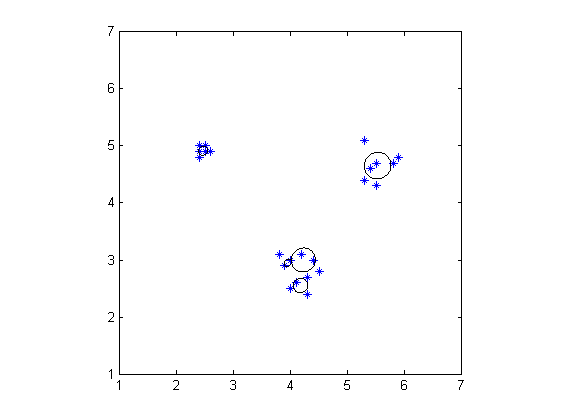
\includegraphics[width=0.5\linewidth]{lab2/emSingle.png}
    \label{fig5:sub1}
}
\subfigure[Expectation Maximization without a single winner. Everything worked out OK.]{
    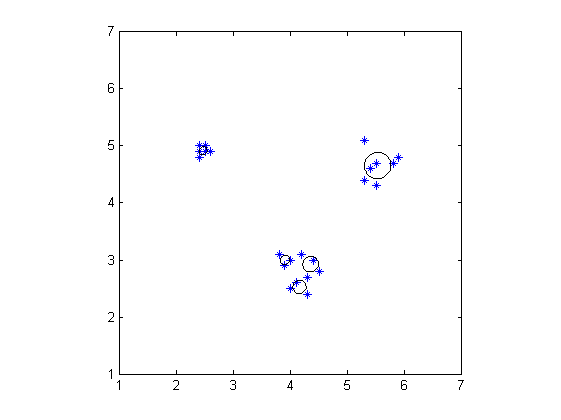
\includegraphics[width=0.5\linewidth]{lab2/emNotSingle.png}
    \label{fig5:sub2}
}
\subfigure[Expectation Maximization with a single winner. We have underfitted the data since we generalise to a area which we have no data in.]{
    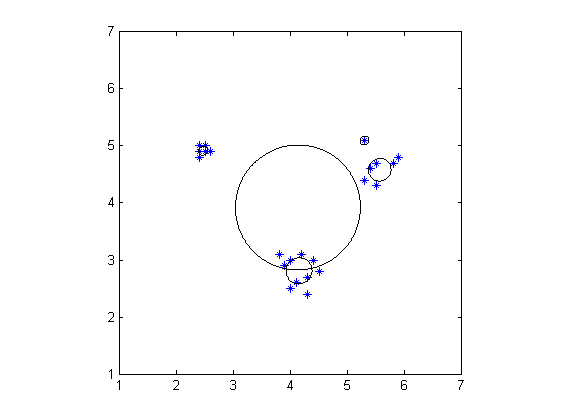
\includegraphics[width=0.5\linewidth]{lab2/emSingleBad.png}
    \label{fig5:sub3}
}
\subfigure[Expectation Maximization with a single winner. Even when we have the same number of units as clusters we can get the same problem.]{
    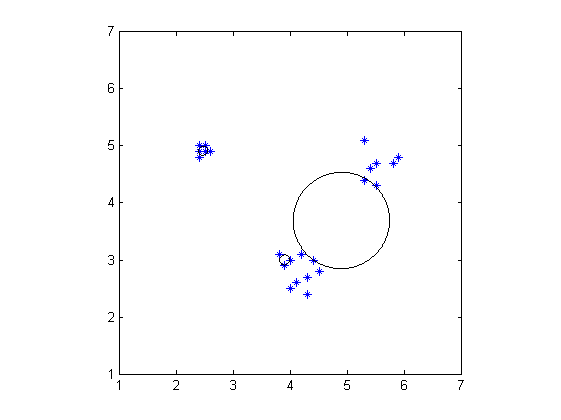
\includegraphics[width=0.5\linewidth]{lab2/emSingleSameClusterAndUnit.png}
    \label{fig5:sub4}
}
\label{fig5}
\caption{}
\end{figure}


\end{itemize}

\clearpage
\section{Ballistics}
\begin{itemize}

\item \textit{When the network har a large learning capacity, there is always the risk of overlearning. If you have time, try reducing the number of units to see if it gets better or worse. You can also test what happens if you low-pass filter the input to get rid of some noise during training. Did you try these improvements? Did it help?}

We see that reducing the number of units in the hidden layer helps since it was overtraining before. We can alos see that reducing the noise with a butterworth lowpass filter doesn't really help to classify the data better. It only helps on the trainig data but not on the validation data. This may have something to do with the fact that we only use a single winner. When we reduce the noise we will have a lower spread of data which may cause a few hidden units to take a lot of the data points, i.e. we may end up with more dead units. Since we have a lot of dead units which are randomly placed they may cause noise in the output data. In that case, as we increase the number of hidden units for the lowpassed data the approximations should become worse as seen in figure \ref{fig6:sub1}

\begin{figure}[h!]
\subfigure[1000 iterations to test impact of hidden units and noise reduction on the approximation function.]{
    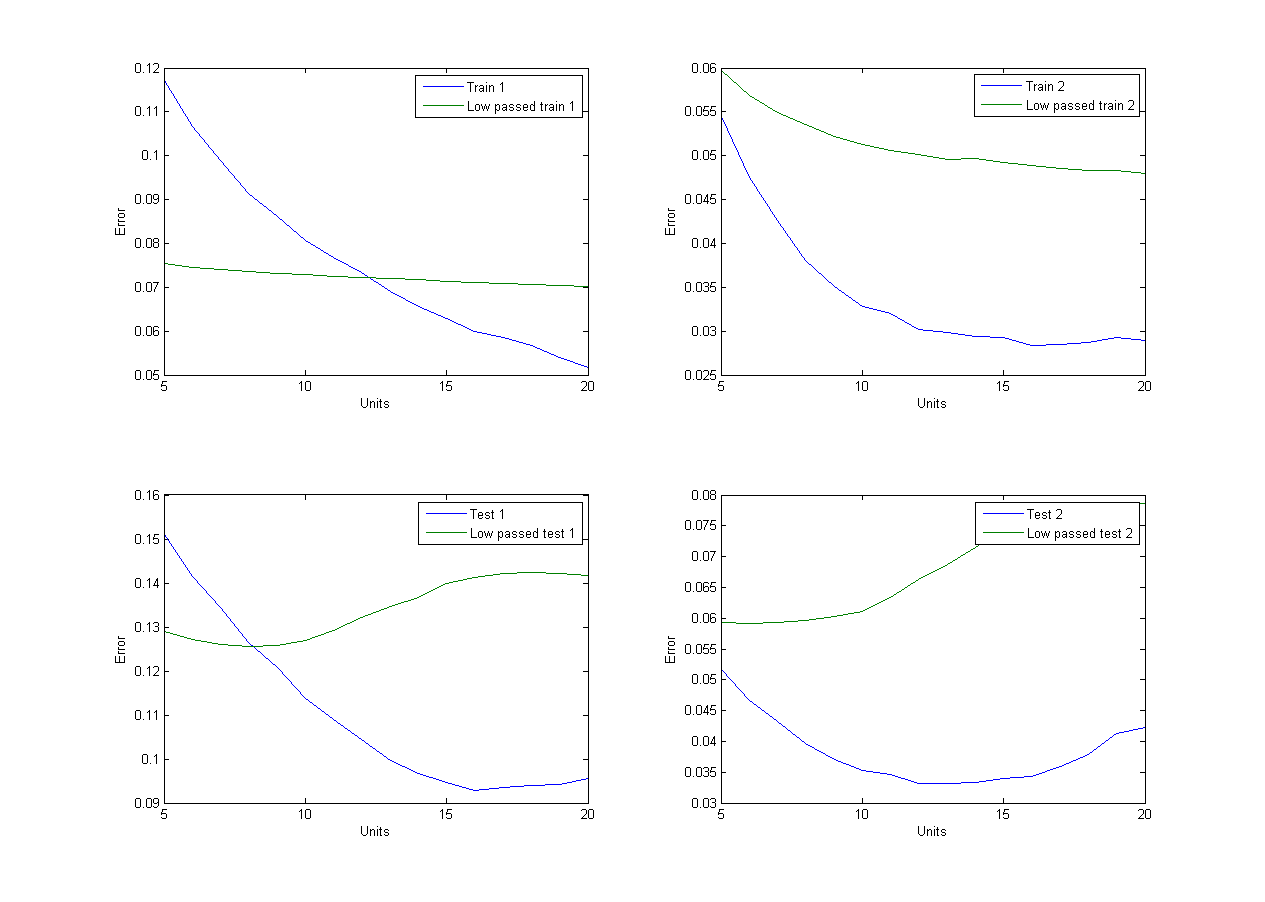
\includegraphics[width=1.0\linewidth]{lab2/noise1000iter.png}
    \label{fig6:sub1}
}
\label{fig6}
\caption{}
\end{figure}

\end{itemize}
\end{document}
